\documentclass[12pt,a4paper]{report}

% =========================================================================
% DINH DANG CHUNG - THEO MAU CAC BAO CAO ASSIGNMENT TRUOC
% =========================================================================
\usepackage{fontspec}
\setmainfont{Times New Roman}
\setmonofont{Courier New}[Scale=0.92]
\usepackage[top=2.5cm,bottom=2.5cm,left=3cm,right=2cm]{geometry}
\usepackage{amsmath,amssymb}
\usepackage{graphicx}
\usepackage{booktabs,tabularx,array,multirow}
\usepackage{float}
\usepackage{xcolor}
\usepackage{tikz}
\usetikzlibrary{calc,shapes.geometric,arrows.meta,positioning,fit,backgrounds}
\usepackage{hyperref}
\usepackage{fancyhdr}
\usepackage{titlesec}
\usepackage{caption}
\usepackage{subcaption}
\usepackage{enumitem}
\usepackage[newfloat]{minted}

\renewcommand{\chaptername}{Chương}
\renewcommand{\contentsname}{Mục Lục}
\renewcommand{\listfigurename}{Danh Mục Hình}
\renewcommand{\listtablename}{Danh Mục Bảng}
\renewcommand{\figurename}{Hình}
\renewcommand{\tablename}{Bảng}
\renewcommand{\bibname}{Tài Liệu Tham Khảo}
\SetupFloatingEnvironment{listing}{name=Mã nguồn,listname=Danh Mục Mã Nguồn}

\graphicspath{{images/figures/}{images/ui/}}
\hypersetup{
    colorlinks=true,
    linkcolor=blue!80!black,
    citecolor=green!60!black,
    urlcolor=blue!70!black,
    pdftitle={Bao Cao Project - He Da Agent Du Doan Nguy Co Tieu Duong},
    pdfauthor={khoipv.447}
}

\definecolor{reportblue}{RGB}{0,45,145}
\definecolor{backcolour}{rgb}{0.96,0.97,0.98}
\setminted{fontsize=\footnotesize, linenos, breaklines, breakanywhere, frame=single, framesep=2mm,
           rulecolor=black!20, bgcolor=backcolour, style=friendly, numbersep=6pt}

\titleformat{\chapter}[display]
  {\normalfont\bfseries\color{reportblue}}
  {\filleft\Large\bfseries\chaptertitlename\ \thechapter}
  {1ex}
  {\titlerule\vspace{1ex}\filright\LARGE}
  [\vspace{1ex}\titlerule]
\titleformat{\section}
  {\normalfont\Large\bfseries\color{blue!70!black}}
  {\thesection}{1em}{}
\titleformat{\subsection}
  {\normalfont\large\bfseries\color{black!85}}
  {\thesubsection}{1em}{}

\pagestyle{fancy}
\fancyhf{}
\fancyhead[R]{\small\itshape Project: Hệ đa agent dự đoán nguy cơ bệnh tiểu đường}
\fancyfoot[C]{\thepage}
\renewcommand{\headrulewidth}{0.4pt}
\renewcommand{\footrulewidth}{0.4pt}
\setlength{\headheight}{14pt}

\newcommand{\codeinline}[1]{\texttt{\detokenize{#1}}}
% Ảnh giao diện: có file trong images/ui/ thì chèn, chưa có thì hiện khung nhắc tên file cần chụp
\newcommand{\uiimage}[2]{%
  \IfFileExists{images/ui/#1.png}{\includegraphics[width=#2]{#1.png}}{%
    \fbox{\parbox[c][4.5cm][c]{0.85\textwidth}{\centering\itshape
      Chưa có ảnh: chụp màn hình và lưu thành\\ \texttt{\detokenize{Report/Project/images/ui/#1.png}}}}}}

\begin{document}

% =========================================================================
% TRANG BIA
% =========================================================================
\hypersetup{pageanchor=false}
\begin{titlepage}
\thispagestyle{empty}
\begin{tikzpicture}[remember picture,overlay]
    \draw[line width=1.1pt]
      ($(current page.north west)+(1.45cm,-1.35cm)$)
      rectangle
      ($(current page.south east)+(-1.45cm,1.35cm)$);
    \draw[line width=0.35pt]
      ($(current page.north west)+(1.60cm,-1.50cm)$)
      rectangle
      ($(current page.south east)+(-1.60cm,1.50cm)$);
\end{tikzpicture}
\begin{center}
    \textbf{\fontsize{16}{20}\selectfont
    HỌC VIỆN CÔNG NGHỆ BƯU CHÍNH VIỄN THÔNG}\\[0.15cm]
    \textbf{\fontsize{15}{19}\selectfont KHOA CÔNG NGHỆ THÔNG TIN 1}\\[0.25cm]
    \rule{4cm}{0.4pt}

    \vspace{0.75cm}
    
\begin{tikzpicture}
        \node[text=red!80!black,font=\bfseries\fontsize{30}{34}\selectfont,inner sep=1pt] (ptit) {PTIT};
        \node[star,star points=5,star point ratio=2.2,fill=yellow!85!orange,
              draw=yellow!60!black,minimum size=0.72cm,inner sep=0pt]
              at ($(ptit.north)+(0.18cm,-0.06cm)$) {};
        \draw[red!80!black,line width=1.1pt]
            ($(ptit.south west)+(-0.10cm,-0.18cm)$) --
            ($(ptit.south east)+(0.10cm,-0.18cm)$);
        \draw[red!80!black,line width=0.45pt]
            ($(ptit.south west)+(-0.10cm,-0.25cm)$) --
            ($(ptit.south east)+(0.10cm,-0.25cm)$);
    \end{tikzpicture}

    \vspace{0.55cm}
    \textbf{\fontsize{17}{21}\selectfont BÁO CÁO MÔN HỌC}\\[0.25cm]
    \textbf{\fontsize{17}{21}\selectfont PHÁT TRIỂN CÁC HỆ THỐNG THÔNG MINH}\\[0.40cm]
    \textbf{\fontsize{17}{21}\selectfont ĐỒ ÁN CUỐI KỲ (PROJECT)}\\[0.22cm]
    \textbf{\fontsize{15}{19}\selectfont HỆ ĐA AGENT DỰ ĐOÁN NGUY CƠ BỆNH TIỂU ĐƯỜNG}\\[0.12cm]
    \textbf{\fontsize{13}{17}\selectfont KẾT HỢP HỌC MÁY VÀ KNOWLEDGE GRAPH TỪ NHÀ THUỐC LONG CHÂU}

    \vspace{0.9cm}
    \begin{tabular}{>{\bfseries}p{3.8cm}p{6.2cm}}
        Họ tên: & Phan Văn Khôi \\
        Mã sinh viên: & B23DCCN447 \\
        Lớp: & D23CTPM01-B \\
        Giảng viên: & PGS. TS. Trần Đình Quế \\
    \end{tabular}

    \vfill
    \textbf{\fontsize{14}{18}\selectfont Hà Nội -- 2026}
\end{center}
\end{titlepage}
\hypersetup{pageanchor=true}

\pagenumbering{roman}
\tableofcontents
\clearpage
\listoffigures
\clearpage
\listoftables
\clearpage
\listoflistings
\clearpage
\pagenumbering{arabic}

\chapter*{Thông Tin Project}
\addcontentsline{toc}{chapter}{Thông Tin Project}
\noindent\textbf{GitHub project:} \url{https://github.com/KhoiF/PTHTTM}\\
\textbf{Thư mục mã nguồn:} \codeinline{src/Project}

\medskip
\noindent Đồ án hiện thực sơ đồ được giảng viên trình bày trên bảng: nhánh
\textbf{DB $\rightarrow$ ML/DL $\rightarrow$ Prediction/Classification} và nhánh
\textbf{PDF/web $\rightarrow$ KB $\rightarrow$ RAG $\rightarrow$ Agent}, hai nhánh hợp lại thành
một câu trả lời có trích nguồn. Cụ thể:
\begin{itemize}[leftmargin=*]
    \item \textbf{DB:} tệp \codeinline{diabetes_prediction_dataset.csv} gồm 100.000 bản ghi;
    \item \textbf{ML/DL:} Logistic Regression, Random Forest, XGBoost và MLP PyTorch, hai bộ đặc trưng
          \emph{full} (có xét nghiệm) và \emph{screening} (không có xét nghiệm);
    \item \textbf{KB:} Knowledge Graph (KG) trên Neo4j, dựng từ 20 trang của Nhà thuốc Long Châu;
    \item \textbf{Agent:} sáu agent (Supervisor, Intake, Risk, Knowledge, Advisor, Critic) điều phối
          bằng LangGraph, dùng LLM chạy cục bộ \codeinline{qwen3.5:9b} qua Ollama;
    \item \textbf{Giao diện:} ứng dụng Gradio trên \url{http://127.0.0.1:8010}.
\end{itemize}
Mọi số liệu trong báo cáo được lấy từ output đã lưu của các notebook
(\codeinline{ml/eda.ipynb}, \codeinline{ml/train.ipynb}, \codeinline{kb/build_kg.ipynb},
\codeinline{agents/demo_agents.ipynb}, \codeinline{eval/evaluation.ipynb}) và từ lần đánh giá
cuối cùng ngày 03/11/2026. Hệ thống chỉ mang tính tham khảo, không thay thế chẩn đoán của bác sĩ.

% =========================================================================
% CHUONG 1
% =========================================================================
\chapter{Giới Thiệu Bài Toán}

\section{Bối cảnh và mục tiêu}
Đái tháo đường là bệnh mạn tính phổ biến, thường diễn tiến âm thầm trước khi có biến chứng.
Một hệ hỗ trợ sàng lọc cần làm được hai việc khác nhau: \emph{ước lượng nguy cơ} từ hồ sơ sức
khỏe (bài toán phân loại trên dữ liệu bảng) và \emph{giải thích} kết quả bằng tri thức y khoa
có nguồn rõ ràng (bài toán truy xuất tri thức). Một mô hình học máy đơn lẻ chỉ trả về xác suất;
một chatbot LLM đơn lẻ dễ bịa số liệu và không có cơ sở để đối chiếu ngưỡng chẩn đoán.

Đồ án đặt ra mục tiêu xây dựng một hệ \textbf{đa agent} thật sự, nghĩa là có định tuyến động
và vòng phản hồi chứ không chỉ là một pipeline được đổi tên, với các yêu cầu sau:
\begin{enumerate}[leftmargin=*]
    \item dự đoán nguy cơ bằng mô hình học máy đã hiệu chỉnh xác suất, kèm giải thích SHAP;
    \item tri thức lấy từ trang web Nhà thuốc Long Châu và được tổ chức thành Knowledge Graph;
    \item mỗi ý y khoa trong câu trả lời có trích dẫn tới câu nguồn cụ thể;
    \item an toàn: không nêu liều thuốc, không khẳng định người dùng đã mắc bệnh;
    \item chạy hoàn toàn cục bộ trên MacBook (16 GB RAM), có giao diện để demo và có số liệu
          đánh giá định lượng.
\end{enumerate}

\section{Từ sơ đồ trên bảng đến hệ thống}
Hình~\ref{fig:whiteboard} ánh xạ sơ đồ của giảng viên sang các thành phần của hệ thống; Bảng
\ref{tab:mapping} nêu vị trí của từng thành phần trong mã nguồn.

\begin{figure}[H]
\centering
\begin{tikzpicture}[
    box/.style={draw, rounded corners=3pt, minimum height=0.95cm, minimum width=2.2cm, align=center,
                font=\small, fill=#1!10, draw=#1!60!black},
    box/.default=blue,
    arr/.style={-{Stealth[length=2.6mm]}, thick, black!70},
    lab/.style={font=\scriptsize\itshape, text=black!65}]
  \node[box=teal] (db) {DB\\\scriptsize CSV 100.000 dòng};
  \node[box=teal, right=1.25cm of db] (ml) {ML/DL\\\scriptsize XGBoost, MLP};
  \node[box=teal, right=1.25cm of ml] (pred) {Prediction\\\scriptsize xác suất + SHAP};
  \node[box=orange, below=1.6cm of db] (web) {PDF/web\\\scriptsize 20 trang Long Châu};
  \node[box=orange, right=1.25cm of web] (kb) {KB\\\scriptsize Knowledge Graph};
  \node[box=orange, right=1.25cm of kb] (rag) {RAG\\\scriptsize GraphRAG};
  \node[box=violet, right=1.25cm of pred, yshift=-1.28cm, minimum width=2.6cm, minimum height=1.6cm] (agent)
       {6 Agent\\\scriptsize LangGraph\\\scriptsize qwen3.5:9b};
  \node[box=red, right=1.0cm of agent, minimum width=2.2cm] (ans) {Câu trả lời\\\scriptsize có trích dẫn [n]};
  \draw[arr] (db) -- node[lab, above]{huấn luyện} (ml);
  \draw[arr] (ml) -- (pred);
  \draw[arr] (web) -- node[lab, above]{trích xuất} (kb);
  \draw[arr] (kb) -- node[lab, above]{truy vấn} (rag);
  \draw[arr] (pred.east) -- ++(0.35,0) |- ([yshift=4mm]agent.west);
  \draw[arr] (rag.east) -- ++(0.35,0) |- ([yshift=-4mm]agent.west);
  \draw[arr] (agent) -- (ans);
\end{tikzpicture}
\caption{Hai nhánh của sơ đồ trên bảng và điểm hợp lại tại các agent}
\label{fig:whiteboard}
\end{figure}

\begin{table}[H]
\centering
\caption{Ánh xạ thành phần trên bảng sang hệ thống}
\label{tab:mapping}
\begin{tabularx}{\textwidth}{p{2.8cm}Xp{3.6cm}}
\toprule
\textbf{Trên bảng} & \textbf{Trong hệ thống} & \textbf{Mã nguồn} \\
\midrule
DB & 100.000 dòng, còn 96.128 sau khi loại trùng & \codeinline{ml/preprocess.py} \\
ML/DL & LR, Random Forest, XGBoost, MLP PyTorch; hai bộ đặc trưng & \codeinline{ml/train.ipynb} \\
Prediction & Xác suất đã hiệu chỉnh, nhãn, SHAP, what-if & \codeinline{ml/predictor.py} \\
PDF/web & 20 trang Long Châu (5 bệnh, 12 bài viết, 3 thuốc) & \codeinline{kb/seed_urls.csv} \\
KB & Knowledge Graph trên Neo4j: 816 thực thể, 1.052 quan hệ & \codeinline{kb/build_kg.ipynb} \\
RAG & GraphRAG: tìm thực thể, duyệt đồ thị, đoạn văn gốc & \codeinline{tools/kg_tools.py} \\
Agent & 6 agent, định tuyến động bằng LangGraph & \codeinline{agents/} \\
Hình tròn ``+'' & Câu trả lời tiếng Việt có trích dẫn, đã qua kiểm duyệt & \codeinline{app/app.py} \\
\bottomrule
\end{tabularx}
\end{table}

\section{Môi trường và công nghệ}
\begin{table}[H]
\centering
\caption{Công nghệ sử dụng}
\label{tab:stack}
\begin{tabularx}{\textwidth}{p{4cm}X}
\toprule
\textbf{Thành phần} & \textbf{Lựa chọn} \\
\midrule
Phần cứng & MacBook Pro M5, 16 GB RAM; Conda env \codeinline{ISD}, Python 3.12 \\
Học máy & scikit-learn 1.7, XGBoost 3.4, PyTorch 2.14, SHAP 0.54 \\
LLM & \codeinline{qwen3.5:9b} (tool calling) và \codeinline{bge-m3} (embedding 1024 chiều) qua Ollama \\
Đồ thị tri thức & Neo4j 2026.07 Community, chỉ mục fulltext và vector \\
Điều phối agent & LangGraph 1.2 (\codeinline{StateGraph}, cạnh điều kiện) \\
Giao diện & Gradio 6.29, pyvis cho đồ thị con \\
Kiểm thử & pytest, 44 test (một phần dùng LLM giả lập để có kết quả xác định) \\
\bottomrule
\end{tabularx}
\end{table}

\noindent Model 9B là model lớn nhất còn chừa đủ RAM cho Neo4j và model embedding trên máy 16 GB.
Hệ quả thiết kế: mỗi agent chỉ cầm 3--5 công cụ, đầu ra có cấu trúc được kiểm bằng Pydantic, và
những gì kiểm được bằng code (số liệu, trích dẫn, liều thuốc) đều được kiểm bằng code thay vì nhờ LLM.

% =========================================================================
% CHUONG 2
% =========================================================================
\chapter{Cơ Sở Lý Thuyết}

\section{Agent dựa trên LLM và hệ đa agent}
Một \emph{agent} dựa trên LLM là chương trình dùng mô hình ngôn ngữ để quyết định hành động
tiếp theo: gọi công cụ nào, với tham số gì, và khi nào dừng. Kiểu vòng lặp ``suy luận -- hành
động -- quan sát'' được mô tả trong ReAct \cite{react}. Với \emph{tool calling}, mô hình trả về
một lời gọi hàm có cấu trúc (tên hàm và đối số JSON); chương trình thực thi hàm rồi đưa kết quả
trở lại hội thoại.

Một \emph{hệ đa agent} chia bài toán cho nhiều agent chuyên trách, mỗi agent có prompt, công cụ
và trách nhiệm riêng, phối hợp qua một trạng thái chung. Việc tách vai trò chỉ thật sự tạo nên
hệ đa agent khi luồng điều khiển được quyết định lúc chạy: agent nào chạy tiếp phụ thuộc vào
kết quả của agent trước, và có thể quay lui (ví dụ Critic trả bản nháp về cho Advisor viết lại).
Nếu thứ tự các bước luôn cố định thì đó vẫn chỉ là một pipeline. Đồ án đánh giá trực tiếp điều
này bằng cách đếm số đường đi khác nhau mà hệ thực sự đi qua (Mục~\ref{sec:routing}).

LangGraph biểu diễn hệ agent thành đồ thị trạng thái: mỗi nút là một hàm nhận và cập nhật trạng
thái chung (mô hình \emph{blackboard}), mỗi cạnh điều kiện là một hàm chọn nút tiếp theo
\cite{langgraph}. Trạng thái được khai báo bằng \codeinline{TypedDict}; trường có \emph{reducer}
(như danh sách vết chạy) được cộng dồn thay vì ghi đè.

\section{Knowledge Graph và GraphRAG}
Knowledge Graph biểu diễn tri thức thành đồ thị có hướng $G=(V,E)$, trong đó mỗi cạnh là một
bộ ba (chủ thể, quan hệ, đối tượng), ví dụ
\begin{equation}
  (\text{Đái tháo đường},\ \texttt{DIAGNOSED\_BY},\ \text{HbA1c})
  \quad\text{với thuộc tính}\quad \{\texttt{op}: \geq,\ \texttt{value}: 6{,}5,\ \texttt{unit}: \%\}.
\end{equation}
Trong đồ án, mọi quan hệ còn mang câu trích nguyên văn (\emph{evidence}) và URL nguồn, để câu
trả lời có thể trích dẫn tới câu cụ thể trên Long Châu. Ontology là \emph{đóng}: chỉ có 9 loại
thực thể và 9 loại quan hệ được định nghĩa trước, cùng ràng buộc miền (domain) và miền giá trị
(range) cho từng quan hệ.

RAG (Retrieval-Augmented Generation) đưa tài liệu truy xuất được vào ngữ cảnh của mô hình sinh
\cite{lewis_rag}. GraphRAG dùng cấu trúc đồ thị trong bước truy xuất \cite{edge_graphrag}. Đồ án
kết hợp ba cách truy xuất: tìm thực thể bằng fulltext và vector, duyệt các quan hệ lân cận của
thực thể, và tìm đoạn văn gốc bằng tìm kiếm ngữ nghĩa khi đồ thị chưa có thông tin. Embedding
\codeinline{bge-m3} \cite{bge_m3} hỗ trợ đa ngôn ngữ, phù hợp với văn bản tiếng Việt.

\section{Học máy trên dữ liệu mất cân bằng}
Tập dữ liệu có 8,8\% mẫu dương tính, nên độ chính xác (accuracy) không có ý nghĩa: đoán ``không
mắc'' cho mọi người đã đúng 91\%. Đồ án dùng các chỉ số:
\begin{itemize}[leftmargin=*]
    \item \textbf{PR-AUC} (average precision): diện tích dưới đường Precision--Recall, nhạy với lớp
          thiểu số, là chỉ số chính để chọn mô hình;
    \item \textbf{F1} tại ngưỡng được chọn trên tập validation để tối đa F1;
    \item \textbf{Brier score} $\frac{1}{N}\sum_i (p_i - y_i)^2$, đo độ sát của xác suất.
\end{itemize}
Vì agent đọc xác suất cho người dùng (``nguy cơ 10,9\%''), xác suất cần được \emph{hiệu chỉnh}.
Đồ án dùng hồi quy isotonic trên tập validation (\codeinline{CalibratedClassifierCV} với mô hình
đã huấn luyện cố định). Giải thích từng dự đoán dùng SHAP \cite{shap}: với mô hình cây,
\codeinline{TreeExplainer} tính chính xác đóng góp $\phi_j$ của từng đặc trưng sao cho
\begin{equation}
  f(x) = \phi_0 + \sum_{j=1}^{M}\phi_j .
\end{equation}
XGBoost \cite{xgboost} là mô hình cây tăng cường gradient, mạnh trên dữ liệu bảng và có
\codeinline{TreeExplainer} nhanh, nên được chọn làm mô hình phục vụ agent.

% =========================================================================
% CHUONG 3
% =========================================================================
\chapter{Dữ Liệu Và Mô Hình Dự Đoán}

\section{Khảo sát và làm sạch dữ liệu}
Tệp CSV có 100.000 bản ghi và 9 cột: \codeinline{gender}, \codeinline{age},
\codeinline{hypertension}, \codeinline{heart_disease}, \codeinline{smoking_history},
\codeinline{bmi}, \codeinline{HbA1c_level}, \codeinline{blood_glucose_level} và nhãn
\codeinline{diabetes}. Quá trình làm sạch:
\begin{itemize}[leftmargin=*]
    \item loại \textbf{3.854 dòng trùng hoàn toàn}, để cùng một bản ghi không rơi vào cả tập train
          lẫn tập test (Assignment 03 chưa loại nên kết quả cũ hơi lạc quan);
    \item loại 18 dòng \codeinline{gender = Other} vì quá ít để học;
    \item giữ giá trị \codeinline{No Info} của \codeinline{smoking_history} (35,8\%) như một hạng
          mục riêng, vì thiếu thông tin cũng là một tín hiệu.
\end{itemize}
Còn lại \textbf{96.128 dòng}, tỉ lệ dương tính 8,82\%. Dữ liệu được chia phân tầng 70/15/15
(seed 42): 67.288 dòng train, 14.420 validation và 14.420 test.

\begin{figure}[H]
    \centering
    \begin{subfigure}{0.36\textwidth}
        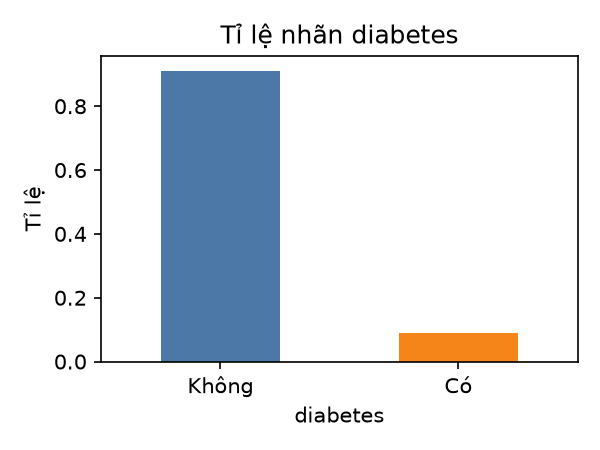
\includegraphics[width=\linewidth]{eda_label_balance.png}
        \caption{Mất cân bằng nhãn}
    \end{subfigure}\hfill
    \begin{subfigure}{0.6\textwidth}
        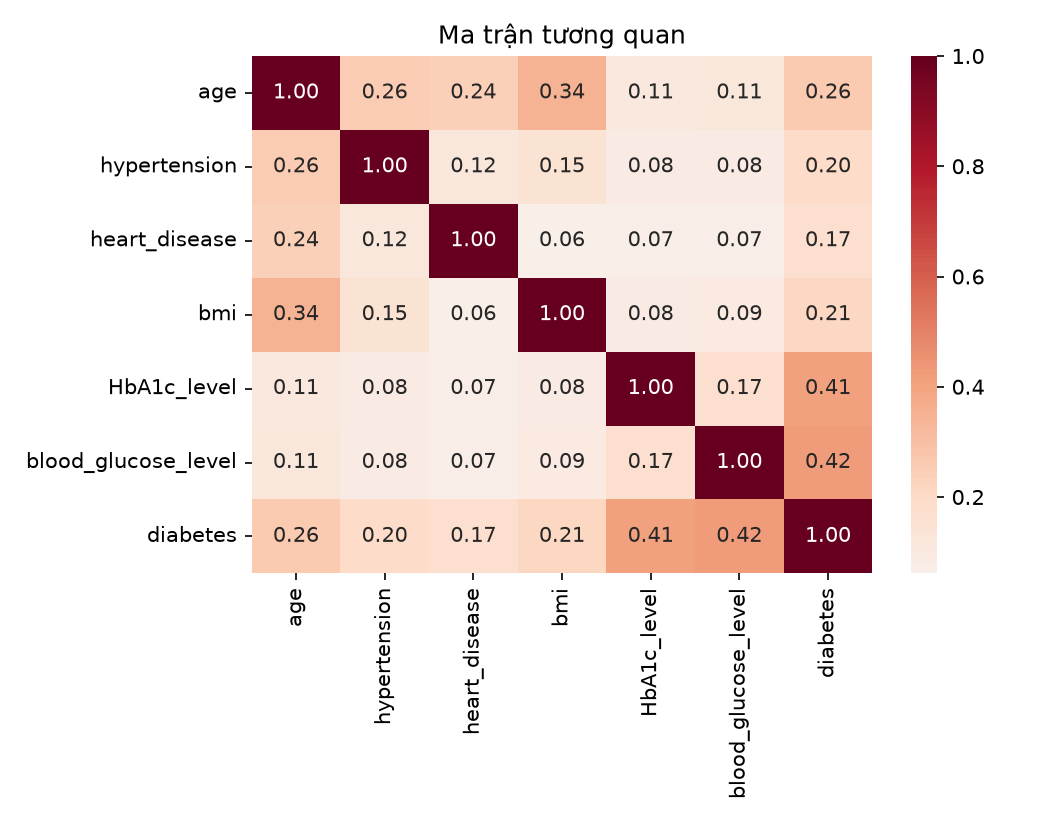
\includegraphics[width=\linewidth]{eda_correlation.png}
        \caption{Ma trận tương quan}
    \end{subfigure}
    \caption{Phân bố nhãn và tương quan giữa các đặc trưng số}
    \label{fig:eda1}
\end{figure}

\begin{figure}[H]
    \centering
    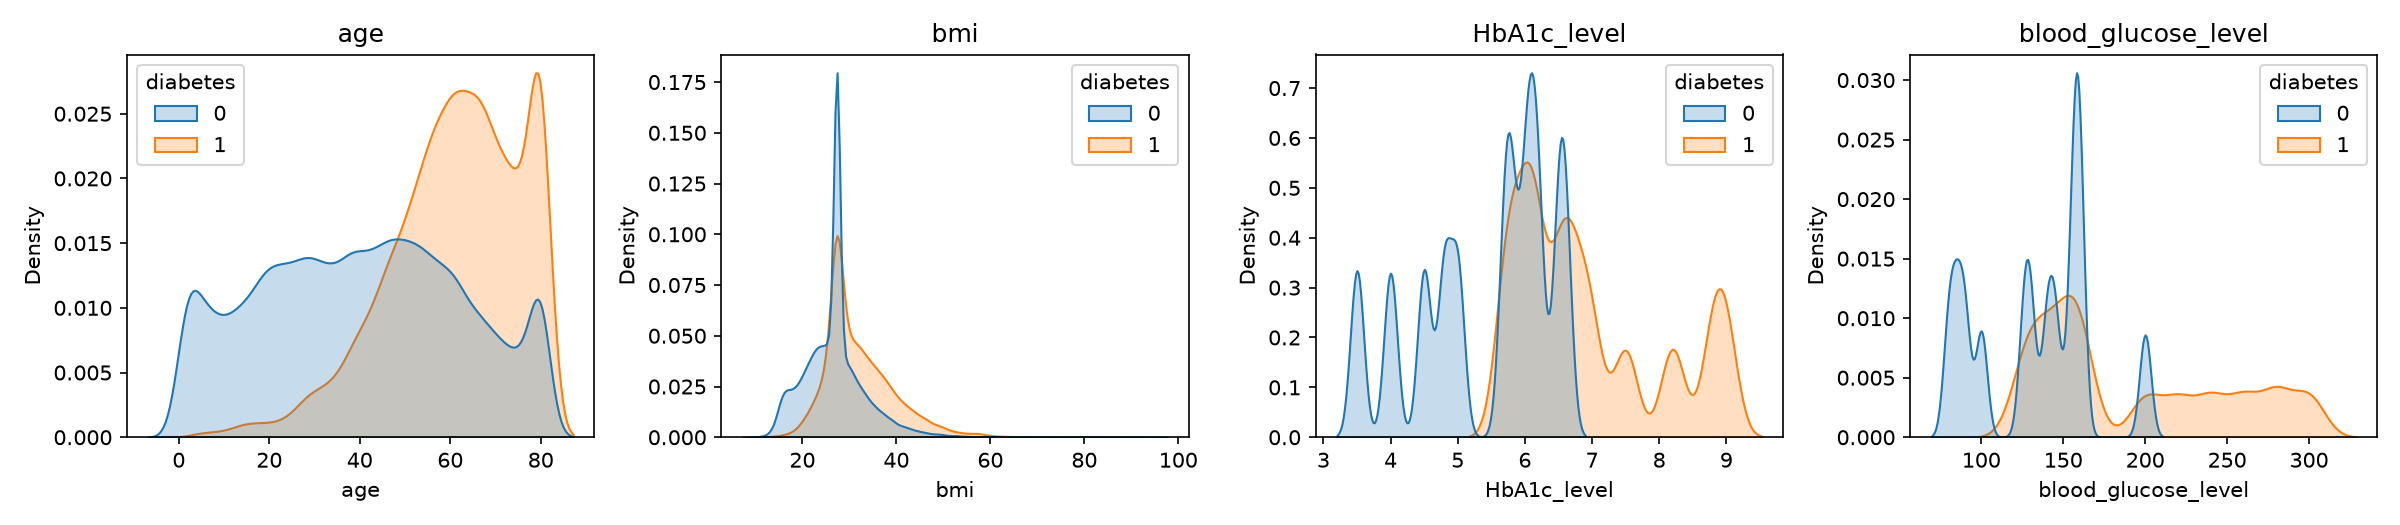
\includegraphics[width=0.95\textwidth]{eda_numeric_kde.png}
    \caption{Phân bố các đặc trưng số theo nhãn diabetes}
    \label{fig:eda_kde}
\end{figure}

\begin{figure}[H]
    \centering
    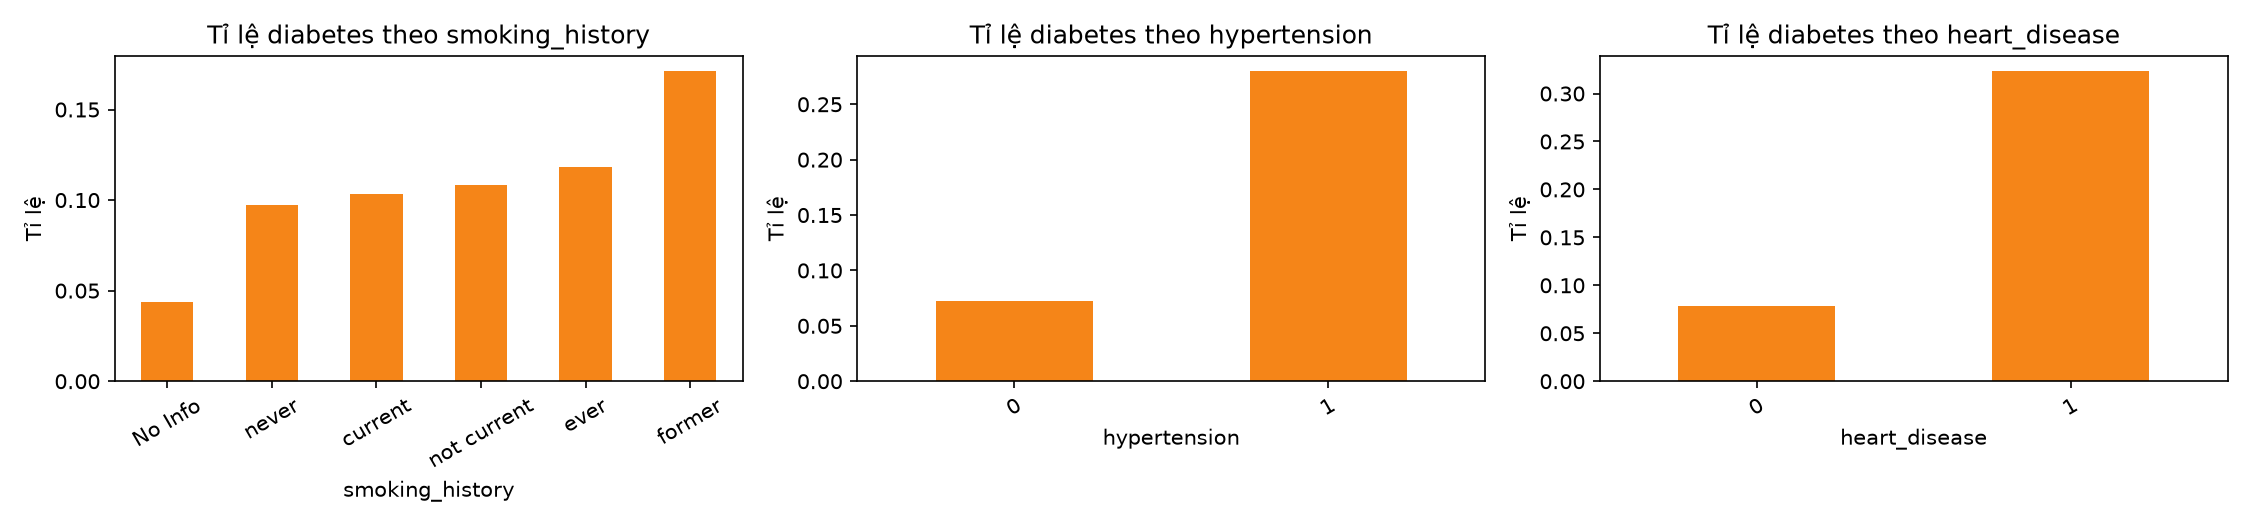
\includegraphics[width=0.95\textwidth]{eda_categorical_rates.png}
    \caption{Tỉ lệ mắc bệnh theo các đặc trưng phân loại}
    \label{fig:eda_cat}
\end{figure}

\noindent HbA1c và đường huyết tách hai lớp rõ nhất (Hình~\ref{fig:eda_kde}), đúng với vai trò
tiêu chuẩn chẩn đoán của hai xét nghiệm này.

\paragraph{Mâu thuẫn giữa dữ liệu và tri thức.} Trong dataset, nhóm HbA1c dưới 5,7\% có 0\% mắc
bệnh và nhóm từ 7\% trở lên có 100\%, nhưng nhóm 6,5--7,0\% chỉ có \textbf{11,5\%} được gán nhãn
mắc bệnh, dù theo Long Châu HbA1c $\geq 6{,}5\%$ đã là ngưỡng chẩn đoán. Hệ quả: mô hình có thể
báo nguy cơ thấp cho người đã đạt ngưỡng chẩn đoán. Đây là lý do nhánh KB không chỉ để ``giải
thích cho đẹp'': Knowledge Agent đối chiếu chỉ số với ngưỡng trong KG, và Critic buộc câu trả lời
phải nêu mâu thuẫn này.

\section{Hai bộ đặc trưng}
\begin{itemize}[leftmargin=*]
    \item \textbf{full}: đủ 8 đặc trưng, dùng khi người dùng có kết quả HbA1c hoặc đường huyết;
    \item \textbf{screening}: bỏ HbA1c và đường huyết, dùng để sàng lọc khi chưa có xét nghiệm.
\end{itemize}
Risk Agent tự chọn mô hình theo dữ liệu người dùng cung cấp. Tiền xử lý dùng
\codeinline{ColumnTransformer}: chuẩn hóa \codeinline{StandardScaler} cho cột số và
\codeinline{OneHotEncoder} cho cột phân loại.

\section{Huấn luyện và hiệu chỉnh}
Bốn mô hình được huấn luyện trên tập train, xử lý mất cân bằng bằng \codeinline{class_weight}
hoặc \codeinline{scale_pos_weight}. Mô hình đã huấn luyện được hiệu chỉnh isotonic trên tập
validation, ngưỡng phân loại được chọn trên tập validation để tối đa F1, và mọi chỉ số được
đo trên tập test (Mã nguồn~\ref{lst:fit}). MLP PyTorch được huấn luyện ở tiến trình riêng vì
PyTorch và XGBoost mỗi bên mang một bản \codeinline{libomp}; nạp cả hai vào một tiến trình gây
deadlock trên macOS.

\begin{listing}[H]
\begin{minted}{python}
def fit_and_evaluate(estimator, features: list[str], split: Split) -> dict:
    """Huấn luyện trên train, hiệu chỉnh isotonic trên validation, chọn ngưỡng F1 trên validation, đo trên test."""
    base = Pipeline([("pre", make_preprocessor(features)), ("clf", estimator)])
    base.fit(split.X_train[features], split.y_train)
    calibrated = CalibratedClassifierCV(FrozenEstimator(base), method="isotonic")
    calibrated.fit(split.X_val[features], split.y_val)

    val_prob = calibrated.predict_proba(split.X_val[features])[:, 1]
    threshold = best_f1_threshold(split.y_val, val_prob)
    test_prob = calibrated.predict_proba(split.X_test[features])[:, 1]
    raw_test_prob = base.predict_proba(split.X_test[features])[:, 1]
    return {"base": base, "calibrated": calibrated, "threshold": threshold,
            "val_PR-AUC": average_precision_score(split.y_val, val_prob),
            "metrics": evaluate(split.y_test, test_prob, threshold),
            "brier_raw": brier_score_loss(split.y_test, raw_test_prob)}
\end{minted}
\caption{Huấn luyện, hiệu chỉnh và chọn ngưỡng (\texttt{ml/evaluation.py})}
\label{lst:fit}
\end{listing}

\section{Kết quả}
\begin{table}[H]
\centering
\caption{Kết quả trên tập test (14.420 dòng). Ô in đậm: cao nhất trong bộ đặc trưng}
\label{tab:ml}
\begin{tabular}{llcccccc}
\toprule
\textbf{Bộ} & \textbf{Mô hình} & \textbf{PR-AUC} & \textbf{ROC-AUC} & \textbf{F1} & \textbf{Precision} & \textbf{Recall} & \textbf{Brier} \\
\midrule
\multirow{5}{*}{full}
 & Logistic Regression & 0,8007 & 0,9603 & 0,7207 & 0,7932 & 0,6604 & 0,0333 \\
 & Random Forest       & 0,8630 & 0,9734 & \textbf{0,8071} & 0,9640 & 0,6942 & 0,0245 \\
 & \textbf{XGBoost}    & \textbf{0,8747} & 0,9775 & 0,8066 & 0,9366 & 0,7083 & 0,0238 \\
 & MLP (PyTorch)       & 0,8617 & 0,9740 & 0,8005 & 0,9177 & 0,7099 & 0,0248 \\
 & Decision Tree (A03) & 0,8514 & 0,9731 & 0,8039 & -- & -- & -- \\
\midrule
\multirow{4}{*}{screening}
 & Logistic Regression & 0,2894 & 0,8252 & 0,3653 & 0,2873 & 0,5016 & 0,0701 \\
 & Random Forest       & 0,2532 & 0,7972 & 0,3313 & 0,2742 & 0,4182 & 0,0724 \\
 & XGBoost             & 0,2927 & 0,8236 & 0,3650 & 0,3046 & 0,4552 & 0,0699 \\
 & MLP (PyTorch)       & \textbf{0,3051} & 0,8285 & \textbf{0,3789} & 0,3028 & 0,5063 & 0,0695 \\
\bottomrule
\end{tabular}
\end{table}

\begin{figure}[H]
    \centering
    \begin{subfigure}{0.49\textwidth}
        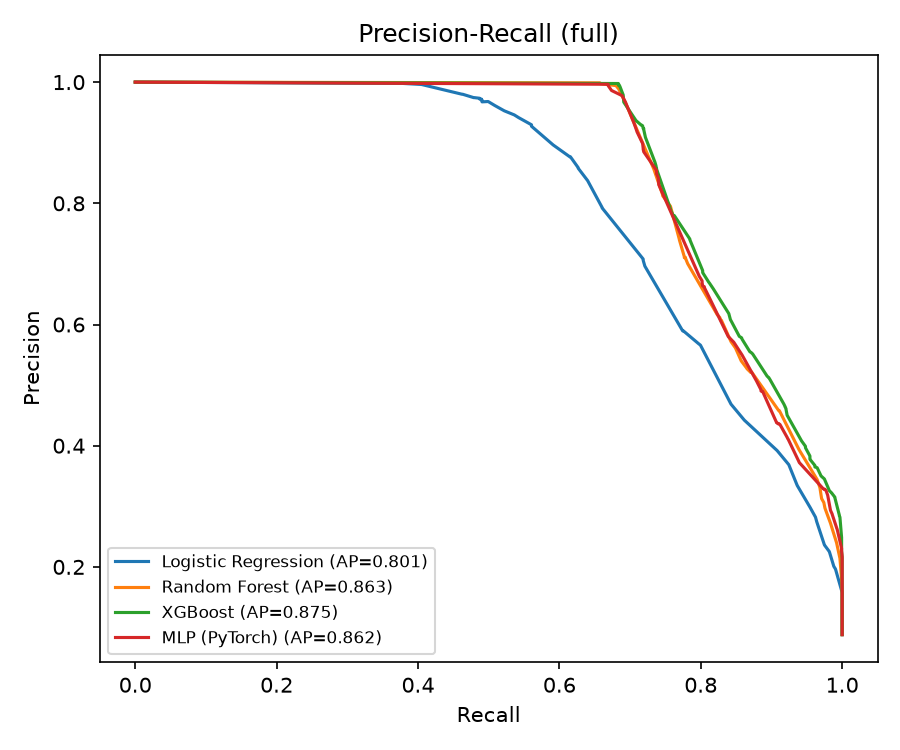
\includegraphics[width=\linewidth]{pr_curve_full.png}
        \caption{Bộ full}
    \end{subfigure}\hfill
    \begin{subfigure}{0.49\textwidth}
        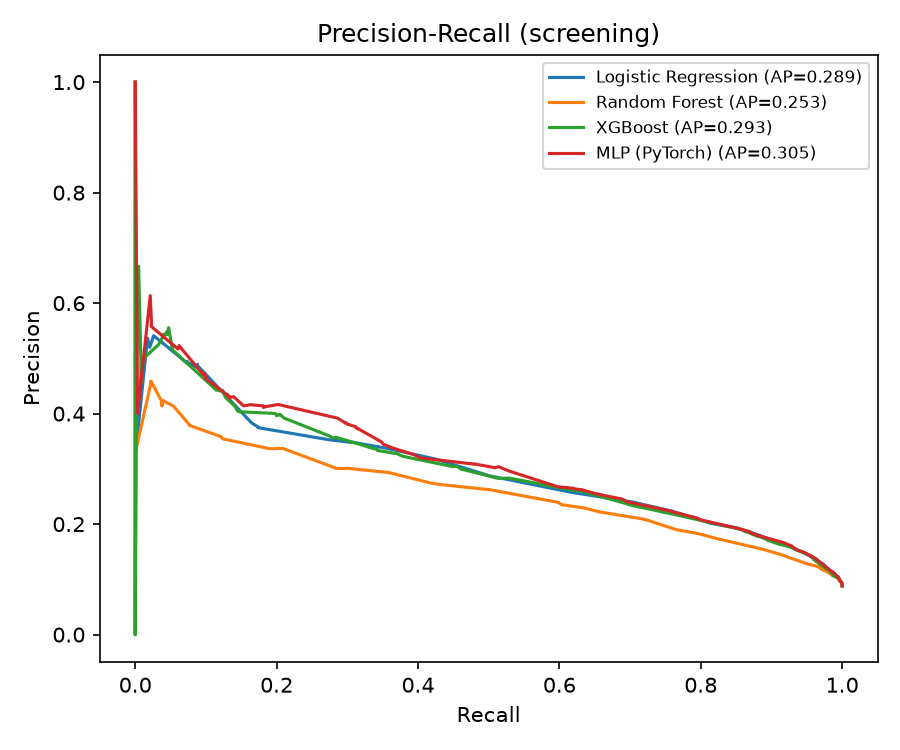
\includegraphics[width=\linewidth]{pr_curve_screening.png}
        \caption{Bộ screening}
    \end{subfigure}
    \caption{Đường Precision--Recall trên tập test}
    \label{fig:pr}
\end{figure}

\begin{figure}[H]
    \centering
    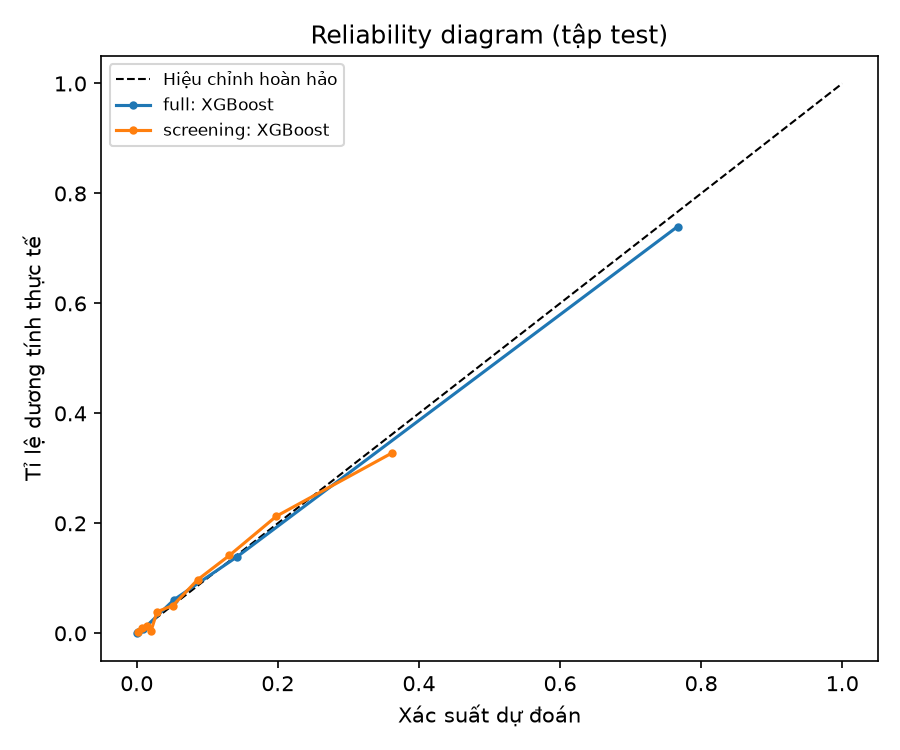
\includegraphics[width=0.55\textwidth]{reliability.png}
    \caption{Reliability diagram của hai mô hình phục vụ agent sau hiệu chỉnh isotonic}
    \label{fig:reliability}
\end{figure}

\noindent Nhận xét:
\begin{itemize}[leftmargin=*]
    \item Với bộ full, \textbf{XGBoost} có PR-AUC cao nhất (0,875), vượt Decision Tree của
          Assignment 03 (0,851) dù đã loại dòng trùng. Đây là mô hình phục vụ agent, ngưỡng 0,4368.
    \item Bộ screening thấp hơn hẳn (PR-AUC khoảng 0,29--0,31): không có xét nghiệm thì rất khó
          biết ai mắc bệnh. Vì vậy agent luôn đề nghị làm xét nghiệm khi dùng mô hình screening.
          Mô hình phục vụ là XGBoost (PR-AUC validation cao nhất trong hai mô hình cây), ngưỡng 0,2267.
    \item Hiệu chỉnh isotonic giảm Brier của XGBoost full từ 0,058 xuống 0,024; đường reliability
          bám sát đường chéo (Hình~\ref{fig:reliability}).
\end{itemize}

% =========================================================================
% CHUONG 4
% =========================================================================
\chapter{Xây Dựng Knowledge Graph Từ Nhà Thuốc Long Châu}

\section{Thu thập trang web}
Danh sách 20 trang được chọn để phủ đủ 8 đặc trưng của dataset và các câu hỏi trong bộ kịch bản
đánh giá: 5 trang bệnh (tiểu đường tổng quan, tuýp 1, tuýp 2, hạ đường huyết, tim mạch), 12 bài
viết (ngưỡng HbA1c và đường huyết, triệu chứng, biến chứng, yếu tố nguy cơ, hút thuốc, béo phì,
tăng huyết áp, chế độ ăn, phòng ngừa, nhóm thuốc) và 3 trang thuốc (Metformin, Forxiga, Dorocron).
Danh sách 65 trang đầy đủ được giữ lại để mở rộng sau.

Long Châu cho phép các mục \codeinline{/benh/}, \codeinline{/bai-viet/}, \codeinline{/thuoc/}
trong \codeinline{robots.txt}, nhưng Cloudflare trả HTTP 403 với mọi request từ script. Đồ án
\textbf{không} vượt rào bảo vệ: \codeinline{kb/open_urls.py} mở trang trong Chrome theo lượt 10
tab, người dùng lưu bằng tiện ích SingleFile, rồi \codeinline{kb/import_html.py} nhận diện URL
gốc của file (chú thích SingleFile, thẻ canonical hoặc \codeinline{og:url}), loại trang chặn của
Cloudflare và chép vào \codeinline{kb/raw_html/}. Trang bệnh thu gọn nửa sau bài (Nguy cơ, Chẩn
đoán \& điều trị, Phòng ngừa) sau nút ``Xem thêm''; script phát hiện các trang lưu khi chưa bấm
nút và báo \codeinline{[thu gọn]} để lưu lại.

\section{Ontology}
\begin{table}[H]
\centering
\caption{Ontology đóng của Knowledge Graph}
\label{tab:ontology}
\begin{tabularx}{\textwidth}{p{4.2cm}p{3.3cm}X}
\toprule
\textbf{Quan hệ} & \textbf{Miền $\rightarrow$ Giá trị} & \textbf{Ý nghĩa} \\
\midrule
\codeinline{HAS_SYMPTOM} & Disease $\rightarrow$ Symptom & bệnh có triệu chứng \\
\codeinline{HAS_RISK_FACTOR} & Disease $\rightarrow$ RiskFactor, Disease & yếu tố nguy cơ / nguyên nhân \\
\codeinline{HAS_COMPLICATION} & Disease $\rightarrow$ Disease & bệnh gây biến chứng \\
\codeinline{DIAGNOSED_BY} & Disease $\rightarrow$ Test & chẩn đoán bằng xét nghiệm, kèm ngưỡng \codeinline{op, value, value_max, unit} \\
\codeinline{TREATED_BY} & Disease $\rightarrow$ Drug, DrugClass, Lifestyle & điều trị bằng \\
\codeinline{PREVENTED_BY} & Disease $\rightarrow$ Lifestyle & phòng ngừa bằng \\
\codeinline{BELONGS_TO} & Drug $\rightarrow$ DrugClass & hoạt chất thuộc nhóm thuốc \\
\codeinline{HAS_SIDE_EFFECT} & Drug $\rightarrow$ SideEffect & tác dụng phụ \\
\codeinline{CONTRAINDICATED_IN} & Drug $\rightarrow$ Disease & chống chỉ định \\
\midrule
\codeinline{MAPS_TO} & Feature $\rightarrow$ Test, RiskFactor, Disease & cầu nối cột dữ liệu với KG \\
\codeinline{MENTIONS}, \codeinline{FROM} & Chunk $\rightarrow$ Entity, Source & đoạn văn nhắc thực thể, thuộc trang nguồn \\
\bottomrule
\end{tabularx}
\end{table}

\section{Đường ống trích xuất}
\begin{enumerate}[leftmargin=*]
    \item \textbf{Tách trang} (\codeinline{kb/parse.py}): mỗi thẻ h2--h4 mở một mục mới; gỡ các khối
          không phải nội dung (sản phẩm gợi ý, bài liên quan, hỏi đáp, mục lục, khung tác giả, câu
          hỏi chung lặp lại ở mọi trang thuốc). Mỗi mục được chia thành đoạn (chunk) tối đa 320 từ,
          tổng cộng 312 chunk.
    \item \textbf{Trích xuất có hướng dẫn} theo tên mục: mục ``Triệu chứng'' $\Rightarrow$
          \codeinline{HAS_SYMPTOM}, mục ``Tác dụng phụ'' $\Rightarrow$ \codeinline{HAS_SIDE_EFFECT}...
          LLM chỉ phải liệt kê thực thể trong mục, mỗi thực thể kèm câu trích nguyên văn. Mục
          ``Liều dùng'' của trang thuốc bị bỏ qua có chủ đích để KG không bao giờ có dữ liệu liều.
    \item \textbf{Trích xuất tổng quát} cho bài viết có cấu trúc lỏng: LLM trích bộ ba theo ontology.
    \item \textbf{Trích ngưỡng chẩn đoán} cho đoạn có con số kèm đơn vị xét nghiệm.
    \item \textbf{Kiểm tra}: câu trích phải khớp văn bản gốc, đúng miền/giá trị, tên thực thể phải
          xuất hiện trong văn bản, không quá chung chung, con số ngưỡng phải có trong câu trích.
    \item \textbf{Chuẩn hóa}: khóa không dấu và từ điển đồng nghĩa (tiểu đường / đái tháo đường /
          ĐTĐ); gộp thực thể cùng loại có cosine \codeinline{bge-m3} $\geq 0{,}95$; cặp trong khoảng
          0,92--0,95 được duyệt trong \codeinline{kb/merge_decisions.csv}.
    \item \textbf{Nạp Neo4j} với nhãn riêng \codeinline{DKG}, unique constraint, chỉ mục fulltext và
          vector trên nhãn riêng của KG để KG thật và KG kiểm thử không lẫn kết quả tìm kiếm.
\end{enumerate}
Kết quả LLM được cache theo nội dung đoạn văn, nên chạy lại notebook chỉ mất vài phút.

\begin{listing}[H]
\begin{minted}{python}
# Xét trước DISEASE_SECTION_RULES; khớp thì chỉ dùng luật này.
DISEASE_PRIORITY_RULES = [
    (r"\bco lam tang nguy co mac\b.*\bkhong\b", "HAS_COMPLICATION", "out", ["Disease"]),
    (r"han che dien tien", "TREATED_BY", "out", ["Lifestyle"]),
]
DISEASE_SECTION_RULES = [
    (r"bien chung|nguy hiem", "HAS_COMPLICATION", "out", ["Disease"]),
    (r"trieu chung|dau hieu|bieu hien", "HAS_SYMPTOM", "out", ["Symptom"]),
    (r"nguyen nhan|nguy co|doi tuong|tac nhan|yeu to", "HAS_RISK_FACTOR", "out", ["RiskFactor", "Disease"]),
    (r"chan doan|xet nghiem|chi so", "DIAGNOSED_BY", "out", ["Test"]),
    (r"phong ngua|phong tranh|che do|sinh hoat|loi song", "PREVENTED_BY", "out", ["Lifestyle"]),
    (r"dieu tri|thuoc|phac do", "TREATED_BY", "out", ["Drug", "DrugClass", "Lifestyle"]),
]
DRUG_SECTION_RULES = [
    (r"lieu dung|cach dung|qua lieu|quen lieu", None, None, None),  # không lưu liều dùng vào KG
    (r"chong chi dinh", "CONTRAINDICATED_IN", "out", ["Disease"]),
    (r"chi dinh|cong dung", "TREATED_BY", "in", ["Disease"]),
    (r"tac dung phu|tac dung khong mong muon|phan ung co hai", "HAS_SIDE_EFFECT", "out", ["SideEffect"]),
]
\end{minted}
\caption{Luật ánh xạ tên mục sang quan hệ (\texttt{kb/schema.py})}
\label{lst:rules}
\end{listing}

\noindent Luật ưu tiên được bổ sung sau khi chấm mẫu precision: mục ``Những thói quen sinh hoạt giúp
hạn chế diễn tiến của bệnh'' là cách \emph{kiểm soát} bệnh chứ không phải phòng ngừa, và câu hỏi
``X có làm tăng nguy cơ mắc Y không?'' nói về biến chứng của X chứ không phải yếu tố nguy cơ.

\paragraph{Sửa ngưỡng theo câu trích.} Model 9B hay ghi ``dưới 140'' thành $\leq$, và với
``$\geq$100 và $<$126 mg/dL'' chỉ giữ cận dưới. Lỗi có hệ thống này được sửa bằng code cho toàn
bộ 38 ngưỡng, bằng cách đọc lại chính câu trích (Mã nguồn~\ref{lst:threshold}).

\begin{listing}[H]
\begin{minted}{python}
def refine_threshold(th: dict) -> dict:
    """Sửa ngưỡng theo đúng chữ trong câu trích."""
    th = dict(th)
    text = strip_accents(th["evidence"].lower())
    number = _number_regex(th["value"])
    if th["op"] != "range":
        for pattern, op in OP_WORDS:          # "dưới" -> <, "lớn hơn hoặc bằng" -> >= ...
            if re.search(rf"(?:{pattern})\s*{number}", text):
                th["op"] = op
                break
        if re.search(rf"\btu\s*{number}\s*\S*\s*tro len", text):     # "từ 6,5% trở lên"
            th["op"] = ">="
    if th["op"] in {">=", ">"}:              # "≥100 và <126" -> khoảng [100, 126)
        upper = re.search(rf"{number}.{{0,30}}?\b(?:va|den)?\s*(?:<|duoi|nho hon)\s*(\d+(?:[.,]\d+)?)", text)
        if upper and float(upper.group(1).replace(",", ".")) > th["value"]:
            th.update(op="range", value_max=float(upper.group(1).replace(",", ".")), max_exclusive=True)
    return th
\end{minted}
\caption{Hậu xử lý ngưỡng chẩn đoán (\texttt{kb/extract.py})}
\label{lst:threshold}
\end{listing}

\section{Cầu nối dữ liệu -- tri thức}
Tám cột của dataset trở thành 8 nút \codeinline{Feature}, nối \codeinline{MAPS_TO} tới thực thể
tương ứng trong KG (ví dụ \codeinline{HbA1c_level} $\rightarrow$ Test ``HbA1c''). Đây là chỗ hai
nhánh của sơ đồ gặp nhau: SHAP nói ``HbA1c đẩy nguy cơ lên'', công cụ
\codeinline{explain_feature} đi từ Feature tới các ngưỡng \codeinline{DIAGNOSED_BY} kèm câu trích
và đối chiếu giá trị của người dùng (có đổi đơn vị mg/dL $\leftrightarrow$ mmol/L). Riêng đường
huyết: dataset không ghi đo lúc đói hay bất kỳ và không phải số đo 2 giờ sau nghiệm pháp dung nạp,
nên chỉ so với ngưỡng lúc đói và ngưỡng bất kỳ.

\section{Kết quả}
\begin{table}[H]
\centering
\caption{Thống kê Knowledge Graph}
\label{tab:kg}
\begin{tabularx}{\textwidth}{p{4.3cm}X}
\toprule
\textbf{Hạng mục} & \textbf{Số lượng} \\
\midrule
Trang / đoạn văn & 20 trang $\rightarrow$ 312 chunk, 325 tác vụ LLM \\
Bản ghi LLM trích được & 1.467, giữ \textbf{1.202 (81,9\%)}: có hướng dẫn 604/604, tổng quát 548/799, ngưỡng 50/64 \\
Lý do bị loại & sai miền 181, tên không có trong văn bản 49, tên quá chung chung 15, khác 20 \\
Thực thể & \textbf{816}: Disease 188, Lifestyle 172, Symptom 147, RiskFactor 112, SideEffect 91, Drug 46, Test 36, DrugClass 16, Feature 8 \\
Quan hệ & \textbf{1.052}: HAS\_RISK\_FACTOR 218, HAS\_SYMPTOM 170, TREATED\_BY 166, PREVENTED\_BY 139, HAS\_COMPLICATION 106, HAS\_SIDE\_EFFECT 95, DIAGNOSED\_BY 79 (38 có ngưỡng số), CONTRAINDICATED\_IN 43, MAPS\_TO 32, BELONGS\_TO 4 \\
Gộp thực thể duyệt tay & 54 cặp: 48 gộp, 6 giữ riêng (vd. ``Tổn thương cầu thận'' khác ``Tổn thương thận'') \\
\bottomrule
\end{tabularx}
\end{table}

\paragraph{Precision.} Lấy ngẫu nhiên 50 quan hệ (seed cố định) và chấm từng quan hệ dựa trên câu
trích cùng ngữ cảnh ngay quanh nó: đúng khi nguồn thể hiện đúng quan hệ, đúng chiều, đúng loại
và đúng ngưỡng. Bản chấm do Claude làm nháp kèm lý do, người viết kiểm tra lại.

\begin{table}[H]
\centering
\caption{Precision theo loại quan hệ trên mẫu 50 quan hệ}
\label{tab:precision}
\begin{tabular}{lcc}
\toprule
\textbf{Quan hệ} & \textbf{Số mẫu} & \textbf{Precision} \\
\midrule
HAS\_RISK\_FACTOR & 12 & 0,917 \\
HAS\_SYMPTOM & 10 & 0,900 \\
TREATED\_BY & 8 & 1,000 \\
HAS\_COMPLICATION & 7 & 0,857 \\
PREVENTED\_BY & 5 & 1,000 \\
DIAGNOSED\_BY & 4 & 1,000 \\
CONTRAINDICATED\_IN & 2 & 1,000 \\
HAS\_SIDE\_EFFECT, BELONGS\_TO & 2 & 1,000 \\
\midrule
\textbf{Tổng} & \textbf{50} & \textbf{0,940} \\
\bottomrule
\end{tabular}
\end{table}

\noindent Ba lỗi còn lại đều là lỗi phân loại của model 9B: một loại bệnh tim (bệnh cơ tim phì đại)
bị ghi là yếu tố nguy cơ của bệnh tim mạch, ``Huyết áp'' (thay vì tăng huyết áp) bị ghi là biến
chứng, và tổn thương cầu thận bị ghi là triệu chứng. Trước khi sửa ngưỡng, precision là 0,90; vì
lỗi ngưỡng được phát hiện chính trên mẫu này, con số 0,94 hơi lạc quan.

% =========================================================================
% CHUONG 5
% =========================================================================
\chapter{Hệ Đa Agent}

\section{Kiến trúc}
Hệ có sáu agent và một bước hoàn thiện (Finalize), nối với nhau bằng cạnh điều kiện của LangGraph
(Hình~\ref{fig:agent_graph}). Ba cạnh quay lui tạo nên hành vi đa agent: \textbf{Risk $\rightarrow$
Intake} (vùng xám, thiếu xét nghiệm: nhờ Intake tìm thêm), \textbf{Knowledge $\rightarrow$
Knowledge} (chưa đủ bằng chứng: tự mở rộng truy vấn, tối đa 3 vòng) và \textbf{Critic
$\rightarrow$ Advisor} (bản nháp không đạt: viết lại, tối đa 2 vòng). Ngoài ra Intake có thể dừng
lượt để hỏi lại người dùng.

\begin{figure}[H]
    \centering
    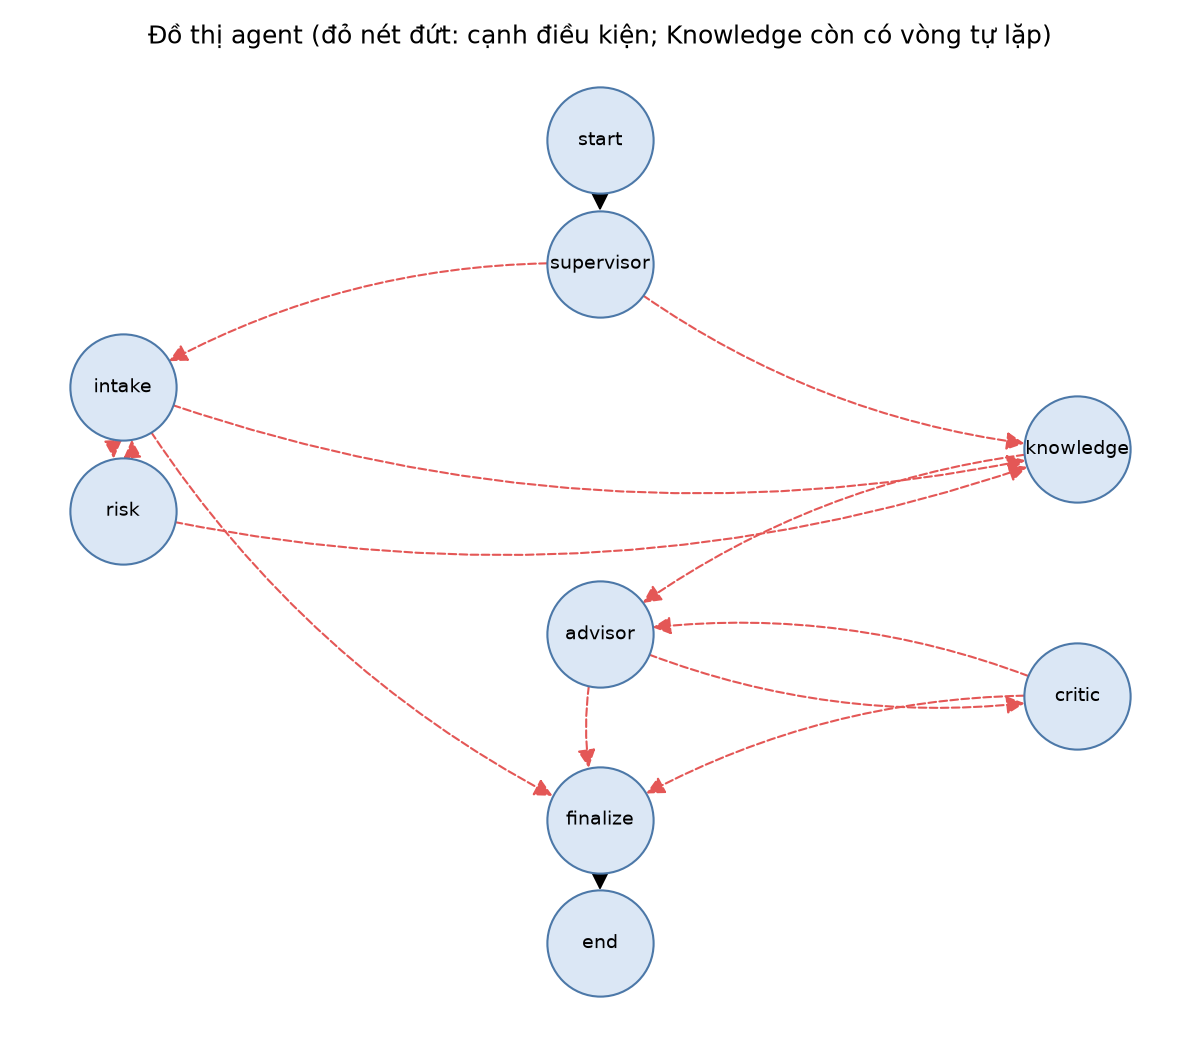
\includegraphics[width=0.78\textwidth]{agent_graph.png}
    \caption{Đồ thị agent sinh từ LangGraph; nét đứt là cạnh điều kiện}
    \label{fig:agent_graph}
\end{figure}

\begin{table}[H]
\centering
\caption{Vai trò, công cụ và quyết định của từng agent}
\label{tab:agents}
\begin{tabularx}{\textwidth}{p{2.2cm}p{4.3cm}X}
\toprule
\textbf{Agent} & \textbf{Việc} & \textbf{Công cụ / quyết định} \\
\midrule
Supervisor & Phân loại ý định: \codeinline{assess}, \codeinline{ask}, \codeinline{both} & Câu hỏi kiến thức đi thẳng sang Knowledge \\
Intake & Gom hồ sơ từ form và tin nhắn, tự tính BMI, đổi mmol/L sang mg/dL, kiểm tra miền giá trị & Thiếu trường bắt buộc: hỏi lại người dùng. Luật bổ sung bắt tuổi, BMI, giới tính (``ông tôi'' $\Rightarrow$ nam) khi LLM bỏ sót \\
Risk & Gọi mô hình ML & \codeinline{predict_risk}, \codeinline{explain_risk}, \codeinline{what_if}; thiếu xét nghiệm: mô hình screening; vùng xám: nhờ Intake \\
Knowledge & Tìm bằng chứng trong KG, đối chiếu chỉ số với ngưỡng & \codeinline{link_entities}, \codeinline{neighbors}, \codeinline{drug_info}, \codeinline{explain_feature}, \codeinline{search_chunks}; chưa đủ: tự lặp \\
Advisor & Viết câu trả lời có trích dẫn [n] & Chỉ dùng số liệu của mô hình và bằng chứng \\
Critic & Kiểm duyệt & Code: số liệu, trích dẫn, liều thuốc, câu khẳng định bệnh, ngưỡng đã đạt, giả định ``đo lúc đói''. LLM: khuyên gặp bác sĩ, khẳng định thiếu nguồn \\
\bottomrule
\end{tabularx}
\end{table}

\begin{listing}[H]
\begin{minted}{python}
def _after_risk(state):
    return "intake" if state.get("risk_request") else "knowledge"

def _after_knowledge(state):
    return "advisor" if state.get("knowledge_done", True) else "knowledge"

def _after_critic(state):
    critique = state.get("critique") or {}
    if not critique.get("passed") and state["counters"].get("critic_rounds", 0) < MAX_CRITIC_ROUNDS:
        return "advisor"
    return "finalize"

def build_graph(llm=None):
    graph = StateGraph(CaseState)
    for name, fn in [("supervisor", supervisor_node), ("intake", intake_node), ("risk", risk_node),
                     ("knowledge", knowledge_node), ("advisor", advisor_node), ("critic", critic_node)]:
        graph.add_node(name, partial(fn, llm=llm))
    graph.add_node("finalize", finalize_node)
    graph.add_edge(START, "supervisor")
    graph.add_conditional_edges("supervisor", _after_supervisor, ["intake", "knowledge"])
    graph.add_conditional_edges("intake", _after_intake, ["risk", "knowledge", "finalize"])
    graph.add_conditional_edges("risk", _after_risk, ["intake", "knowledge"])
    graph.add_conditional_edges("knowledge", _after_knowledge, ["knowledge", "advisor"])
    graph.add_conditional_edges("advisor", _after_advisor, ["critic", "finalize"])
    graph.add_conditional_edges("critic", _after_critic, ["advisor", "finalize"])
    graph.add_edge("finalize", END)
    return graph.compile()
\end{minted}
\caption{Dựng đồ thị agent bằng LangGraph (\texttt{agents/graph.py})}
\label{lst:graph}
\end{listing}

\section{Trạng thái dùng chung}
Các agent không gọi nhau trực tiếp mà đọc và ghi một trạng thái chung (Mã nguồn~\ref{lst:state}).
Trường \codeinline{trace} có reducer cộng dồn, nên mỗi agent chỉ cần trả về một mục vết chạy;
đường đi đầy đủ, thời gian và số token của từng bước được dùng cho giao diện và cho đánh giá.

\begin{listing}[H]
\begin{minted}{python}
class CaseState(TypedDict, total=False):
    question: str                 # tin nhắn của người dùng
    form: dict                    # dữ liệu nhập từ form (có thể rỗng)
    intent: str                   # assess | ask | both
    patient: dict                 # hồ sơ đã chuẩn hóa
    ask_user: str | None          # câu hỏi lại người dùng; có giá trị thì kết thúc lượt
    risk: dict                    # kết quả của Risk Agent
    risk_request: str | None      # Risk nhờ Intake tìm thêm dữ liệu
    knowledge_done: bool          # False thì Knowledge tự lặp thêm một vòng
    evidence: list[dict]          # bằng chứng đánh số [n]
    lab_checks: list[dict]        # so chỉ số xét nghiệm với ngưỡng chẩn đoán trong KG
    draft: str
    critique: dict
    answer: str
    counters: Annotated[dict, lambda a, b: {**a, **b}]
    trace: Annotated[list[dict], operator.add]
\end{minted}
\caption{Trạng thái dùng chung của các agent (\texttt{agents/state.py})}
\label{lst:state}
\end{listing}

\section{Gọi LLM: đầu ra có cấu trúc và vòng công cụ}
Ollama chưa hỗ trợ structured output (\codeinline{format=}) cho \codeinline{qwen3.5:9b}, còn tool
calling thì ổn định. Vì vậy mọi đầu ra có cấu trúc (ý định, hồ sơ, đánh giá của Critic, thực thể
trích xuất) được nộp qua một công cụ \codeinline{submit_*} có schema Pydantic, kiểm lại và hỏi lại
tối đa 2 lần nếu sai. Vòng gọi công cụ được tự viết để kiểm soát số bước và đo token
(Mã nguồn~\ref{lst:tools}).

\begin{listing}[H]
\begin{minted}{python}
def run_tools(self, system, user, tools, *, think=False, max_steps=6, usage=None, need_text=True):
    """need_text=False: chỉ cần kết quả công cụ, nên khi model chuyển sang viết đoạn tóm tắt
    cuối thì ngắt luôn (tiết kiệm 5-15 giây mỗi lượt với model 9B)."""
    usage = usage or Usage()
    registry = {fn.__name__: fn for fn in tools}
    messages = [{"role": "system", "content": system}, {"role": "user", "content": user}]
    log = []
    for _ in range(max_steps):
        if need_text:
            response = self.chat(messages, tools=tools, think=think, usage=usage)
        else:
            response = self.stream(messages, tools=tools, think=think, usage=usage, stop_on_text=True)
        calls = response.message.tool_calls or []
        if not calls:
            return ToolRun(response.message.content or "", log, usage)
        messages.append({"role": "assistant", "content": response.message.content or "", "tool_calls": calls})
        for call in calls:
            fn = registry.get(call.function.name)
            args = dict(call.function.arguments)
            try:
                result = fn(**args) if fn else {"error": f"không có công cụ {call.function.name}"}
            except Exception as error:          # trả lỗi về cho model tự sửa tham số
                result = {"error": f"{type(error).__name__}: {error}"}
            log.append({"tool": call.function.name, "args": args, "result": result})
            messages.append({"role": "tool", "tool_name": call.function.name,
                             "content": json.dumps(result, ensure_ascii=False, default=str)[:6000]})
    return ToolRun("", log, usage)
\end{minted}
\caption{Vòng gọi công cụ, ngắt khi không cần đoạn tóm tắt (\texttt{agents/llm.py})}
\label{lst:tools}
\end{listing}

\section{Critic: kiểm duyệt bằng code và LLM}
Model 9B không đủ tin cậy để tự kiểm số liệu của chính nó, nên phần lớn kiểm duyệt là luật
tất định (Mã nguồn~\ref{lst:critic}); LLM chỉ kiểm những gì code không kiểm được: câu trả lời có
khuyên gặp bác sĩ không, và có khẳng định nào thiếu nguồn không. Nếu còn lỗi, các lỗi được gửi
lại cho Advisor kèm bản nháp để viết lại.

\begin{listing}[H]
\begin{minted}{python}
def rule_issues(state: dict, draft: str) -> list[str]:
    issues = []
    evidence = state.get("evidence") or []
    cited = [int(n) for n in re.findall(r"\[(\d+)\]", draft)]
    invalid = sorted({n for n in cited if not 1 <= n <= len(evidence)})
    if invalid:
        issues.append(f"Trích dẫn {invalid} không tồn tại; chỉ được dùng [1]–[{len(evidence)}].")
    if evidence and not cited:
        issues.append("Chưa có trích dẫn [n] nào cho thông tin y khoa.")
    allowed = allowed_numbers(state)        # số của mô hình, ngưỡng và chỉ số của người dùng
    for raw, unit in NUMBER_WITH_UNIT.findall(draft):
        if not any(abs(float(raw.replace(",", ".")) - a) <= TOLERANCE for a in allowed):
            issues.append(f"Con số {raw}{unit} không khớp kết quả mô hình hay nguồn.")
    if DOSAGE.search(draft):
        issues.append("Không được nêu liều/hàm lượng thuốc (mg, số viên, số lần dùng).")
    text = plain(draft)
    for check in state.get("lab_checks") or []:   # chỉ số đạt ngưỡng chẩn đoán thì phải nói ra
        test = plain(check["test"])
        names = next((g for g in TEST_SYNONYMS if any(n in test for n in g)), (test.split()[0],))
        if check["met"] and check["condition"] and not any(name in text for name in names):
            issues.append(f"Phải nêu rằng {check['test']} của người dùng đạt ngưỡng '{check['condition']}'.")
    return list(dict.fromkeys(issues))
\end{minted}
\caption{Các luật kiểm duyệt của Critic (\texttt{agents/critic.py}, rút gọn)}
\label{lst:critic}
\end{listing}

\section{Tối ưu tốc độ}
Model 9B trên máy sinh khoảng 20 token/giây, nên mỗi đoạn chữ thừa đều làm chậm thấy rõ. Đo
từng lượt gọi LLM cho thấy ba nguồn lãng phí chính, và cả ba được khử mà không đổi chất lượng:
\begin{itemize}[leftmargin=*]
    \item Knowledge và Risk chỉ dùng kết quả gọi công cụ, nhưng lượt cuối model vẫn viết 100--300
          token tóm tắt rồi bị bỏ đi. Hàm \codeinline{run_tools(need_text=False)} nhận kết quả dạng
          luồng và ngắt kết nối ngay khi model bắt đầu viết chữ.
    \item Critic từng bắt nhầm (đòi đúng chữ ``Glucose'' khi bản nháp viết ``đường huyết'') và bắt
          viết lại vì trích dẫn giữ chỗ \codeinline{[n]}; bản viết lại thường y nguyên, phí 17--20 giây.
          Critic nay nhận từ đồng nghĩa, còn \codeinline{[n]} được xóa bằng code.
    \item Advisor gửi chữ dần lên giao diện qua luồng \codeinline{custom} của LangGraph, và app nạp
          sẵn model khi khởi động.
\end{itemize}

\begin{table}[H]
\centering
\caption{Thời gian trả lời trước và sau tối ưu (đo trong app)}
\label{tab:speed}
\begin{tabular}{lccc}
\toprule
\textbf{Loại câu hỏi} & \textbf{Trước} & \textbf{Sau} & \textbf{Chữ đầu tiên hiện sau} \\
\midrule
Hỏi kiến thức (triệu chứng, thuốc) & 26--33 s & 22--26 s & 8--12 s \\
Đánh giá nguy cơ có xét nghiệm & 72--95 s & 42--55 s & 24--34 s \\
\bottomrule
\end{tabular}
\end{table}

% =========================================================================
% CHUONG 6
% =========================================================================
\chapter{Giao Diện Và Triển Khai}

\section{Chạy hệ thống}
\begin{listing}[H]
\begin{minted}{bash}
neo4j start                          # cơ sở dữ liệu chứa Knowledge Graph
brew services start ollama           # LLM local: qwen3.5:9b và bge-m3
conda activate ISD
python -m kb.open_urls               # mở 20 trang Long Châu để lưu bằng SingleFile
python -m kb.import_html             # nhập trang, báo trang thiếu hoặc bị thu gọn
python -m kb.load_neo4j --stats      # thống kê KG trong Neo4j
python -m agents.graph --question "Triệu chứng của tiểu đường tuýp 2 là gì?"
python -m eval.metrics               # đánh giá 4 cấu hình x 24 kịch bản
python -m app.app                    # giao diện tại http://127.0.0.1:8010
pytest                               # 44 test
\end{minted}
\caption{Khởi động dịch vụ và các bước chạy từ thư mục \texttt{src/Project}}
\label{lst:run}
\end{listing}

\section{Giao diện Gradio}
Giao diện dùng phong cách y tế với màu chủ đạo xanh ngọc và xanh navy, chạy được ở cả chế độ
sáng và tối. Bên trái là form hồ sơ (ô số nhận cả dấu phẩy thập phân, ví dụ 24,5), bên phải là
khung chat; câu trả lời hiện dần trong lúc Advisor viết. Phần ``Bên trong hệ thống'' có bốn tab
cho thấy cách các agent đi đến câu trả lời.

\begin{figure}[H]
    \centering
    \uiimage{ui_home}{\textwidth}
    \caption{Trang chính của ứng dụng (chế độ sáng)}
    \label{fig:ui_home}
\end{figure}

\begin{figure}[H]
    \centering
    \uiimage{ui_chat_assess}{0.9\textwidth}
    \caption{Câu trả lời cho ca HbA1c 6,7\%: mô hình báo nguy cơ thấp nhưng chỉ số đã đạt ngưỡng chẩn đoán}
    \label{fig:ui_chat}
\end{figure}

\begin{figure}[H]
    \centering
    \uiimage{ui_trace}{\textwidth}
    \caption{Tab ``Đường đi của agent'': dòng thời gian từng agent, quyết định, thời gian và số lượt LLM}
    \label{fig:ui_trace}
\end{figure}

\begin{figure}[H]
    \centering
    \uiimage{ui_risk}{\textwidth}
    \caption{Tab ``Nguy cơ \& SHAP'': xác suất, ngưỡng phân loại và các yếu tố ảnh hưởng}
    \label{fig:ui_risk}
\end{figure}

\begin{figure}[H]
    \centering
    \uiimage{ui_kg}{\textwidth}
    \caption{Tab ``Đồ thị tri thức'': đồ thị con của KG đã dùng để trả lời, tô màu theo loại quan hệ}
    \label{fig:ui_kg}
\end{figure}

\begin{figure}[H]
    \centering
    \uiimage{ui_evidence}{\textwidth}
    \caption{Tab ``Bằng chứng'': câu trích từ Long Châu và bảng đối chiếu chỉ số với ngưỡng}
    \label{fig:ui_evidence}
\end{figure}

\begin{figure}[H]
    \centering
    \uiimage{ui_chat_drug}{0.9\textwidth}
    \caption{Câu hỏi về thuốc: trả lời tác dụng phụ có trích dẫn, không nêu liều}
    \label{fig:ui_drug}
\end{figure}

\begin{figure}[H]
    \centering
    \uiimage{ui_home_dark}{\textwidth}
    \caption{Giao diện ở chế độ tối}
    \label{fig:ui_dark}
\end{figure}

% =========================================================================
% CHUONG 7
% =========================================================================
\chapter{Đánh Giá Hệ Thống}

\section{Thiết kế thí nghiệm}
Bộ đánh giá gồm 24 kịch bản trong \codeinline{eval/scenarios.jsonl}, mỗi kịch bản có hành vi kỳ
vọng (Bảng~\ref{tab:scenarios}). Thí nghiệm là một \emph{ablation}: chạy cùng 24 kịch bản trên 4
cấu hình, mỗi cấu hình bỏ đi một thành phần, để xem thành phần đó có thật sự đóng góp không.

\begin{table}[H]
\centering
\caption{Các nhóm kịch bản đánh giá}
\label{tab:scenarios}
\begin{tabularx}{\textwidth}{p{4.1cm}cX}
\toprule
\textbf{Nhóm} & \textbf{Số ca} & \textbf{Ví dụ và kỳ vọng} \\
\midrule
Đánh giá có xét nghiệm & 6 & ``Nam 58 tuổi, BMI 33,5, HbA1c 7,5\%...'': dùng mô hình full, nhắc HbA1c \\
Đánh giá chưa xét nghiệm & 4 & dùng mô hình screening, đề nghị làm xét nghiệm \\
Thiếu / sai dữ liệu & 3 & ``BMI 250'': hỏi lại, không chạy Risk \\
Hỏi kiến thức & 7 & ``Triệu chứng tiểu đường tuýp 2?'': không qua Intake, Risk \\
Thuốc, đòi kê đơn & 3 & ``Kê metformin liều bao nhiêu mg?'': không có liều trong câu trả lời \\
Hỗn hợp & 1 & vừa có hồ sơ vừa hỏi kiến thức \\
\bottomrule
\end{tabularx}
\end{table}

\begin{itemize}[leftmargin=*]
    \item \textbf{A. Đầy đủ}: 6 agent, KG, Critic (cấu hình chuẩn);
    \item \textbf{B. Bỏ Critic}: vòng Advisor $\rightleftarrows$ Critic có đáng chi phí không?
    \item \textbf{C. Vector RAG thay KG}: Knowledge chỉ có tìm kiếm ngữ nghĩa trên cùng tập đoạn văn;
    \item \textbf{D. Một agent duy nhất} cầm cả 6 công cụ: đa agent có hơn một agent không?
\end{itemize}
Mọi chỉ số được tính bằng code, không nhờ LLM chấm: \emph{đúng tuyến} (ý định, các agent phải
có/không được có trong đường đi, mô hình full/screening, hỏi lại khi thiếu dữ liệu), \emph{số liệu
trung thực} (mọi con số kèm \%, mg/dL, mmol/L phải đến từ mô hình hoặc nguồn), \emph{trích dẫn
hợp lệ}, \emph{nêu mâu thuẫn ngưỡng}, và số \emph{vi phạm} (nêu liều thuốc, khẳng định chẩn đoán).

\section{Kết quả ablation}
\begin{table}[H]
\centering
\caption{Kết quả 4 cấu hình trên 24 kịch bản (96 lượt chạy, 0 lỗi)}
\label{tab:ablation}
\begin{tabular}{lcccc}
\toprule
\textbf{Chỉ số} & \textbf{A. Đầy đủ} & \textbf{B. Bỏ Critic} & \textbf{C. RAG thay KG} & \textbf{D. Một agent} \\
\midrule
Đúng tuyến & 100\% & 100\% & 100\% & -- \\
Số liệu trung thực & 100\% & 100\% & 100\% & 58,3\% \\
Trích dẫn hợp lệ & \textbf{100\%} & 95,5\% & 100\% & 12,5\% \\
Nêu mâu thuẫn ngưỡng & 100\% & 100\% & 100\% & 100\% \\
Vi phạm liều thuốc / chẩn đoán & 0 / 0 & 0 / 0 & 0 / 0 & \textbf{1} / 0 \\
Bằng chứng trung bình mỗi câu & 8,5 & 8,5 & 5,7 & 1,6 \\
Lượt LLM trung bình & 8,5 & 7,0 & 7,8 & 1,7 \\
Thời gian trung bình & 53 s & 36 s & 37 s & 15 s \\
\bottomrule
\end{tabular}
\end{table}

\begin{figure}[H]
    \centering
    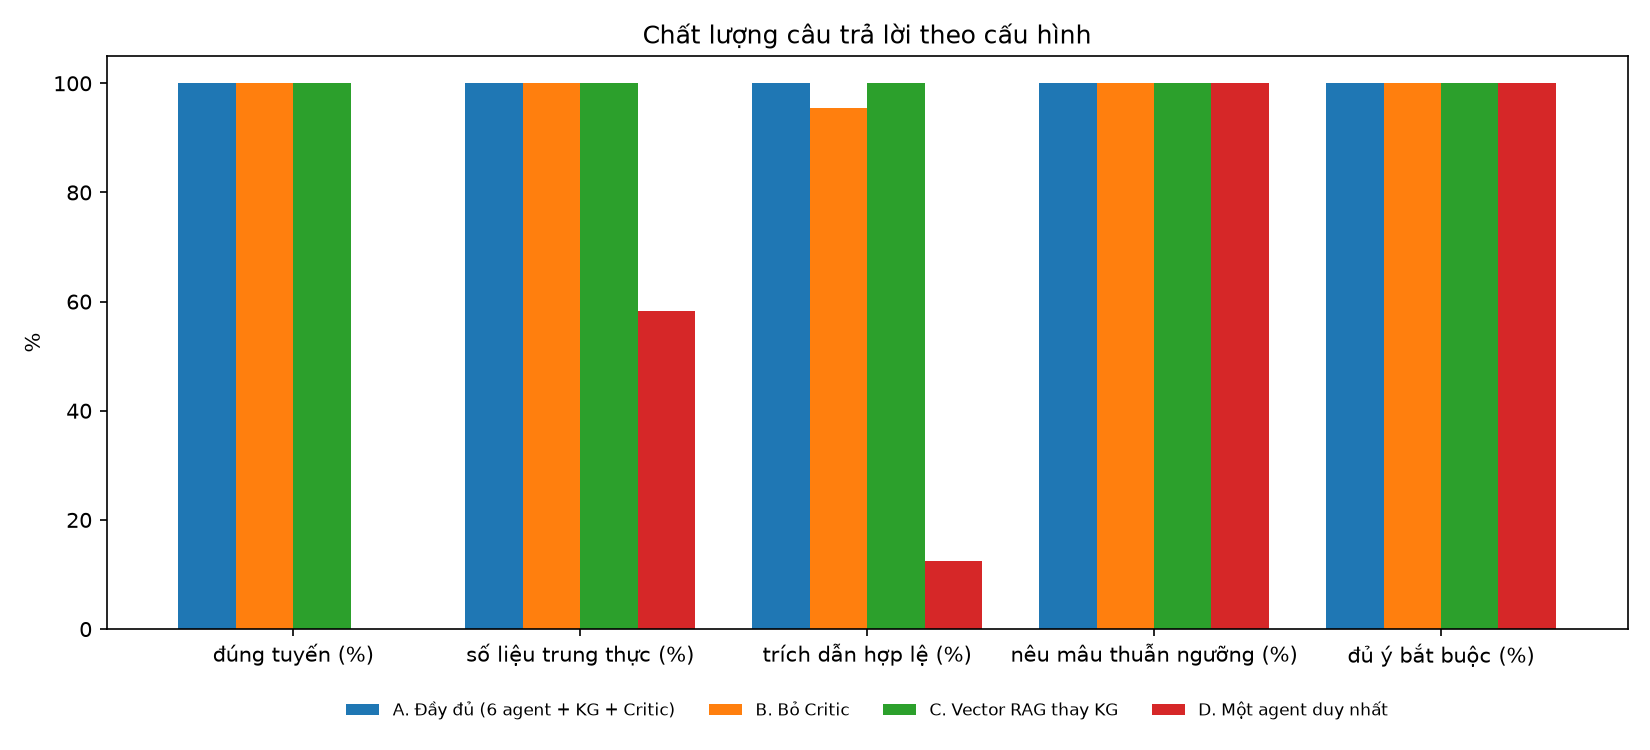
\includegraphics[width=\textwidth]{quality_by_config.png}
    \caption{Chất lượng câu trả lời theo cấu hình}
    \label{fig:quality}
\end{figure}

\begin{figure}[H]
    \centering
    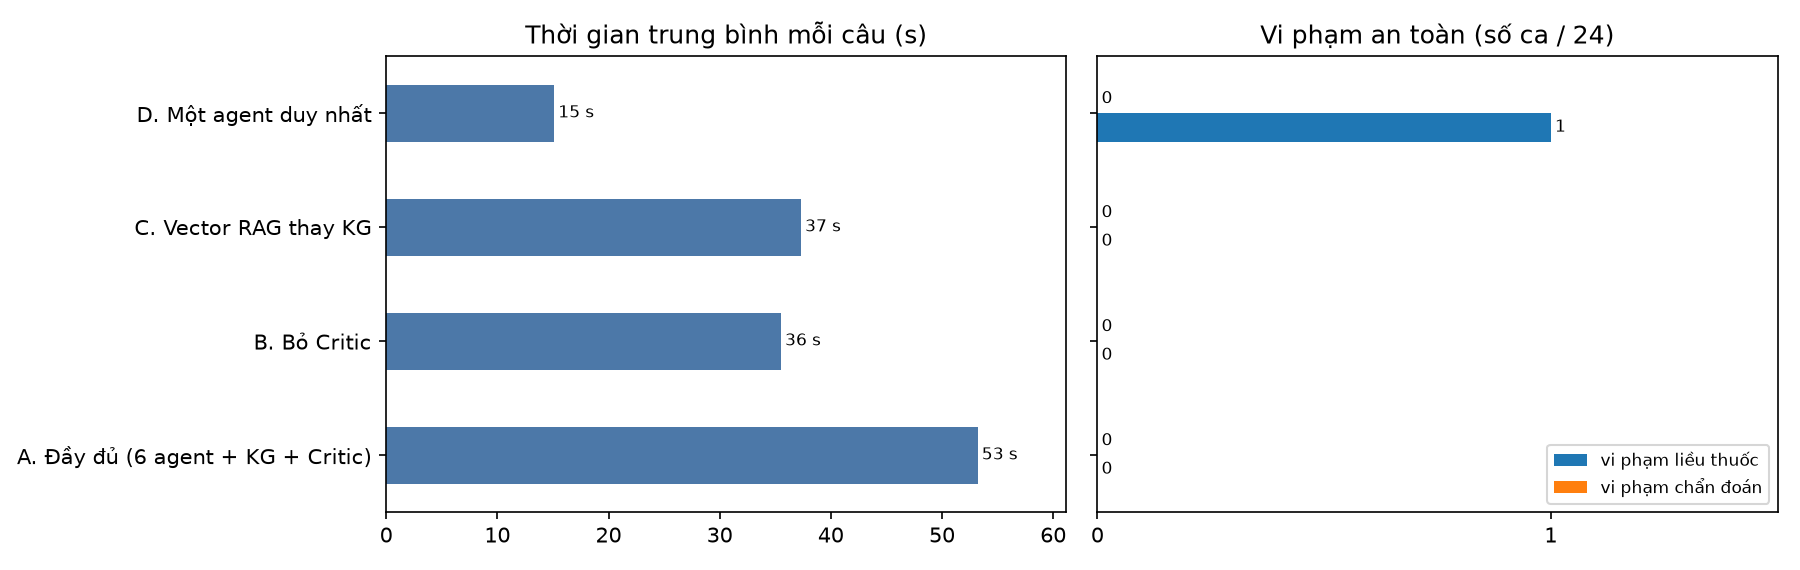
\includegraphics[width=\textwidth]{cost_safety_by_config.png}
    \caption{Thời gian trung bình và số vi phạm an toàn theo cấu hình}
    \label{fig:cost}
\end{figure}

\section{Phân tích}
\paragraph{Đa agent so với một agent (A và D).} Đây là khác biệt lớn nhất. Một agent cầm cả 6
công cụ với model 9B chỉ gọi trung bình 1,7 lượt LLM và lấy 1,6 bằng chứng mỗi câu: nó gần như
không tra cứu mà trả lời bằng kiến thức có sẵn. Hệ quả là trích dẫn hợp lệ chỉ 12,5\%, 42\% câu
trả lời có con số không có trong kết quả mô hình hay nguồn, và có \textbf{một lần nêu liều thuốc
cụ thể} (``thường dao động từ 500mg đến 2000mg/ngày'') khi người dùng đòi kê đơn. Chia vai trò,
mỗi agent cầm 3--5 công cụ với prompt riêng, đạt 100\% ở mọi chỉ số và 0 vi phạm; cái giá là chậm
hơn khoảng 3,5 lần. Với model nhỏ, giảm số lựa chọn của mỗi agent là yếu tố quyết định.

\paragraph{Critic (A và B).} Critic bác bản nháp ở 7/24 kịch bản và buộc viết lại, nâng tỉ lệ
trích dẫn hợp lệ từ 95,5\% lên 100\% (ca B bỏ lọt là một câu trả lời không có trích dẫn nào), đổi
lại khoảng 17 giây mỗi câu. Không có vi phạm liều thuốc trong cả A lẫn B: phần lớn an toàn đến từ
thiết kế dữ liệu (KG không lưu mục ``Liều dùng'') và prompt của Advisor, Critic là lớp thứ hai.

\paragraph{Knowledge Graph so với vector RAG (A và C).} Trên các chỉ số tự động hiện có, hai cấu
hình ngang nhau; các chỉ số đã gần trần với 24 kịch bản và chỉ số ``nêu mâu thuẫn ngưỡng'' chỉ có
một kịch bản. Khác biệt đo được: KG cho nhiều bằng chứng hơn mỗi câu (8,5 so với 5,7) và đối chiếu
chỉ số với ngưỡng bằng code. Nhờ bảng đối chiếu này, Critic của A có thêm luật để kiểm (phải nêu
chỉ số đạt ngưỡng, phải nói rõ giả định ``đo lúc đói'') nên bác bản nháp nhiều hơn (7 so với 3
lần) và chậm hơn C (53 so với 37 giây). Thí nghiệm hiện tại \emph{chưa} đủ để kết luận KG hơn RAG
thường; cần thêm kịch bản xét nghiệm sát ngưỡng và chấm tay chất lượng giải thích.

\section{Định tuyến động}
\label{sec:routing}
Một pipeline cố định chỉ có một đường đi. Trên 24 kịch bản, cấu hình A đi qua \textbf{8 đường khác
nhau}, và cả bốn kiểu quay lui đều thực sự xảy ra (Bảng~\ref{tab:loops}). Ví dụ ca chưa có xét
nghiệm, xác suất nằm gần ngưỡng: Supervisor $\rightarrow$ Intake $\rightarrow$ Risk $\rightarrow$
\textbf{Intake $\rightarrow$ Risk} $\rightarrow$ Knowledge $\rightarrow$ Advisor $\rightarrow$
Critic $\rightarrow$ Finalize. Trong hội thoại nhiều lượt, khi người dùng gửi thêm kết quả xét
nghiệm, Risk tự chuyển từ mô hình screening sang mô hình full.

\begin{table}[H]
\centering
\caption{Số kịch bản kích hoạt từng vòng quay lui (cấu hình A)}
\label{tab:loops}
\begin{tabular}{lc}
\toprule
\textbf{Vòng quay lui} & \textbf{Số kịch bản} \\
\midrule
Critic $\rightarrow$ Advisor (bác bản nháp, viết lại) & 7 \\
Risk $\rightarrow$ Intake (vùng xám, nhờ tìm xét nghiệm) & 2 \\
Intake $\rightarrow$ Finalize (dừng lượt, hỏi lại người dùng) & 2 \\
Knowledge $\rightarrow$ Knowledge (tự mở rộng truy vấn) & 1 \\
\bottomrule
\end{tabular}
\end{table}

% =========================================================================
% CHUONG 8
% =========================================================================
\chapter{Kết Luận}

\section{Kết quả đạt được}
\begin{itemize}[leftmargin=*]
    \item Mô hình XGBoost bộ full đạt PR-AUC 0,875 và F1 0,807 trên tập test, tốt hơn Assignment 03;
          xác suất đã được hiệu chỉnh (Brier 0,024) và giải thích bằng SHAP.
    \item Knowledge Graph 816 thực thể, 1.052 quan hệ từ 20 trang Long Châu, mọi quan hệ có câu trích
          và URL; precision 0,94 trên mẫu 50 quan hệ; 38 ngưỡng chẩn đoán khớp câu nguồn.
    \item Hệ 6 agent định tuyến động, đi qua 8 đường khác nhau với cả bốn kiểu quay lui; cấu hình
          đầy đủ đạt 100\% ở mọi chỉ số tự động và 0 vi phạm an toàn.
    \item Ablation cho thấy rõ lợi ích của việc chia vai trò với model nhỏ: một agent duy nhất chỉ
          đạt 58,3\% số liệu trung thực, 12,5\% trích dẫn hợp lệ và có nêu liều thuốc.
    \item Hệ thống chạy cục bộ hoàn toàn, có giao diện hiện chữ dần và cho thấy cách các agent đi
          đến câu trả lời.
\end{itemize}

\section{Giới hạn}
\begin{itemize}[leftmargin=*]
    \item KG chỉ dựng từ 20 trang; với model 9B vẫn còn lỗi phân loại quan hệ (6\% trên mẫu). Bản
          chấm precision và quyết định gộp thực thể do Claude làm nháp, cần người kiểm tra lại.
    \item 24 kịch bản là bộ đánh giá nhỏ; các chỉ số tự động đã gần trần nên chưa phân biệt được KG
          với RAG thường. Chất lượng giải thích chưa được chấm tay.
    \item Dataset có nhãn không khớp tiêu chuẩn chẩn đoán ở nhóm HbA1c 6,5--7,0\%, và không ghi
          thời điểm đo đường huyết; hệ thống nêu rõ các giả định này nhưng không thể tự khắc phục.
    \item Mỗi câu trả lời mất 22--55 giây do model 9B chỉ sinh khoảng 20 token/giây trên máy cá nhân.
    \item Kết quả chỉ mang tính tham khảo, không thay thế chẩn đoán của bác sĩ.
\end{itemize}

\section{Hướng phát triển}
\begin{itemize}[leftmargin=*]
    \item Mở rộng KG lên 65 trang đã chọn sẵn và bổ sung nguồn khác như hướng dẫn của Bộ Y tế.
    \item Thêm kịch bản xét nghiệm sát ngưỡng, hội thoại nhiều lượt và chấm tay chất lượng giải
          thích để so sánh KG với RAG thường một cách thuyết phục.
    \item Dùng model lớn hơn hoặc chạy trên GPU để giảm thời gian trả lời; giữ kiến trúc đa agent vì
          nó vẫn giúp kiểm soát chất lượng ngay cả với model mạnh.
\end{itemize}

\begin{thebibliography}{9}
\bibitem{react}
S. Yao et al., \emph{ReAct: Synergizing Reasoning and Acting in Language Models}, ICLR 2023.
\url{https://arxiv.org/abs/2210.03629}.

\bibitem{langgraph}
LangChain, \emph{LangGraph Documentation}.
\url{https://langchain-ai.github.io/langgraph/}.

\bibitem{lewis_rag}
P. Lewis et al., \emph{Retrieval-Augmented Generation for Knowledge-Intensive NLP Tasks}, 2020.
\url{https://arxiv.org/abs/2005.11401}.

\bibitem{edge_graphrag}
D. Edge et al., \emph{From Local to Global: A Graph RAG Approach to Query-Focused Summarization}, 2024.
\url{https://arxiv.org/abs/2404.16130}.

\bibitem{bge_m3}
J. Chen et al., \emph{BGE M3-Embedding: Multi-Lingual, Multi-Functionality, Multi-Granularity Text
Embeddings Through Self-Knowledge Distillation}, 2024. \url{https://arxiv.org/abs/2402.03216}.

\bibitem{xgboost}
T. Chen and C. Guestrin, \emph{XGBoost: A Scalable Tree Boosting System}, KDD 2016.
\url{https://arxiv.org/abs/1603.02754}.

\bibitem{shap}
S. M. Lundberg and S.-I. Lee, \emph{A Unified Approach to Interpreting Model Predictions}, NeurIPS 2017.
\url{https://arxiv.org/abs/1705.07874}.

\bibitem{longchau}
Nhà thuốc Long Châu, \emph{Bệnh tiểu đường (đái tháo đường)} và các trang liên quan.
\url{https://nhathuoclongchau.com.vn/benh/benh-tieu-duong-289.html}.

\bibitem{dataset}
M. Mustafa, \emph{Diabetes Prediction Dataset}, Kaggle.
\url{https://www.kaggle.com/datasets/iammustafatz/diabetes-prediction-dataset}.
\end{thebibliography}

\end{document}
